\documentclass[1p]{elsarticle_modified}
%\bibliographystyle{elsarticle-num}

%\usepackage[colorlinks]{hyperref}
%\usepackage{abbrmath_seonhwa} %\Abb, \Ascr, \Acal ,\Abf, \Afrak
\usepackage{amsfonts}
\usepackage{amssymb}
\usepackage{amsmath}
\usepackage{amsthm}
\usepackage{scalefnt}
\usepackage{amsbsy}
\usepackage{kotex}
\usepackage{caption}
\usepackage{subfig}
\usepackage{color}
\usepackage{graphicx}
\usepackage{xcolor} %% white, black, red, green, blue, cyan, magenta, yellow
\usepackage{float}
\usepackage{setspace}
\usepackage{hyperref}

\usepackage{tikz}
\usetikzlibrary{arrows}

\usepackage{multirow}
\usepackage{array} % fixed length table
\usepackage{hhline}

%%%%%%%%%%%%%%%%%%%%%
\makeatletter
\renewcommand*\env@matrix[1][\arraystretch]{%
	\edef\arraystretch{#1}%
	\hskip -\arraycolsep
	\let\@ifnextchar\new@ifnextchar
	\array{*\c@MaxMatrixCols c}}
\makeatother %https://tex.stackexchange.com/questions/14071/how-can-i-increase-the-line-spacing-in-a-matrix
%%%%%%%%%%%%%%%

\usepackage[normalem]{ulem}

\newcommand{\msout}[1]{\ifmmode\text{\sout{\ensuremath{#1}}}\else\sout{#1}\fi}
%SOURCE: \msout is \stkout macro in https://tex.stackexchange.com/questions/20609/strikeout-in-math-mode

\newcommand{\cancel}[1]{
	\ifmmode
	{\color{red}\msout{#1}}
	\else
	{\color{red}\sout{#1}}
	\fi
}

\newcommand{\add}[1]{
	{\color{blue}\uwave{#1}}
}

\newcommand{\replace}[2]{
	\ifmmode
	{\color{red}\msout{#1}}{\color{blue}\uwave{#2}}
	\else
	{\color{red}\sout{#1}}{\color{blue}\uwave{#2}}
	\fi
}

\newcommand{\Sol}{\mathcal{S}} %segment
\newcommand{\D}{D} %diagram
\newcommand{\A}{\mathcal{A}} %arc


%%%%%%%%%%%%%%%%%%%%%%%%%%%%%5 test

\def\sl{\operatorname{\textup{SL}}(2,\Cbb)}
\def\psl{\operatorname{\textup{PSL}}(2,\Cbb)}
\def\quan{\mkern 1mu \triangleright \mkern 1mu}

\theoremstyle{definition}
\newtheorem{thm}{Theorem}[section]
\newtheorem{prop}[thm]{Proposition}
\newtheorem{lem}[thm]{Lemma}
\newtheorem{ques}[thm]{Question}
\newtheorem{cor}[thm]{Corollary}
\newtheorem{defn}[thm]{Definition}
\newtheorem{exam}[thm]{Example}
\newtheorem{rmk}[thm]{Remark}
\newtheorem{alg}[thm]{Algorithm}

\newcommand{\I}{\sqrt{-1}}
\begin{document}

%\begin{frontmatter}
%
%\title{Boundary parabolic representations of knots up to 8 crossings}
%
%%% Group authors per affiliation:
%\author{Yunhi Cho} 
%\address{Department of Mathematics, University of Seoul, Seoul, Korea}
%\ead{yhcho@uos.ac.kr}
%
%
%\author{Seonhwa Kim} %\fnref{s_kim}}
%\address{Center for Geometry and Physics, Institute for Basic Science, Pohang, 37673, Korea}
%\ead{ryeona17@ibs.re.kr}
%
%\author{Hyuk Kim}
%\address{Department of Mathematical Sciences, Seoul National University, Seoul 08826, Korea}
%\ead{hyukkim@snu.ac.kr}
%
%\author{Seokbeom Yoon}
%\address{Department of Mathematical Sciences, Seoul National University, Seoul, 08826,  Korea}
%\ead{sbyoon15@snu.ac.kr}
%
%\begin{abstract}
%We find all boundary parabolic representation of knots up to 8 crossings.
%
%\end{abstract}
%\begin{keyword}
%    \MSC[2010] 57M25 
%\end{keyword}
%
%\end{frontmatter}

%\linenumbers
%\tableofcontents
%
\newcommand\colored[1]{\textcolor{white}{\rule[-0.35ex]{0.8em}{1.4ex}}\kern-0.8em\color{red} #1}%
%\newcommand\colored[1]{\textcolor{white}{ #1}\kern-2.17ex	\textcolor{white}{ #1}\kern-1.81ex	\textcolor{white}{ #1}\kern-2.15ex\color{red}#1	}

{\Large $\underline{12a_{0212}~(K12a_{0212})}$}

\setlength{\tabcolsep}{10pt}
\renewcommand{\arraystretch}{1.6}
\vspace{1cm}\begin{tabular}{m{100pt}>{\centering\arraybackslash}m{274pt}}
\multirow{5}{120pt}{
	\centering
	\includegraphics[width=112pt]{../../../GIT/diagram.site/Diagrams/png/1013_12a_0212.png}\\
\ \ \ A knot diagram\footnotemark}&
\allowdisplaybreaks
\textbf{Linearized knot diagam} \\
\cline{2-2}
 &
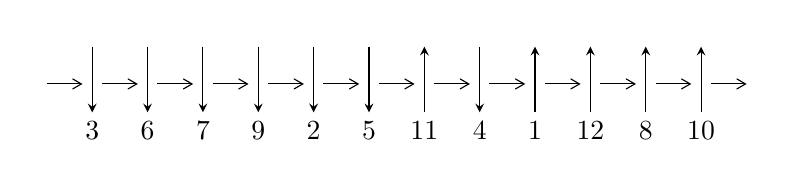
\begin{tikzpicture}[x=20pt, y=17pt]
	% nodes
	\node (C0) at (0, 0) {};
	\node (C1) at (1, 0) {};
	\node (C1U) at (1, +1) {};
	\node (C1D) at (1, -1) {3};

	\node (C2) at (2, 0) {};
	\node (C2U) at (2, +1) {};
	\node (C2D) at (2, -1) {6};

	\node (C3) at (3, 0) {};
	\node (C3U) at (3, +1) {};
	\node (C3D) at (3, -1) {7};

	\node (C4) at (4, 0) {};
	\node (C4U) at (4, +1) {};
	\node (C4D) at (4, -1) {9};

	\node (C5) at (5, 0) {};
	\node (C5U) at (5, +1) {};
	\node (C5D) at (5, -1) {2};

	\node (C6) at (6, 0) {};
	\node (C6U) at (6, +1) {};
	\node (C6D) at (6, -1) {5};

	\node (C7) at (7, 0) {};
	\node (C7U) at (7, +1) {};
	\node (C7D) at (7, -1) {11};

	\node (C8) at (8, 0) {};
	\node (C8U) at (8, +1) {};
	\node (C8D) at (8, -1) {4};

	\node (C9) at (9, 0) {};
	\node (C9U) at (9, +1) {};
	\node (C9D) at (9, -1) {1};

	\node (C10) at (10, 0) {};
	\node (C10U) at (10, +1) {};
	\node (C10D) at (10, -1) {12};

	\node (C11) at (11, 0) {};
	\node (C11U) at (11, +1) {};
	\node (C11D) at (11, -1) {8};

	\node (C12) at (12, 0) {};
	\node (C12U) at (12, +1) {};
	\node (C12D) at (12, -1) {10};
	\node (C13) at (13, 0) {};

	% arrows
	\draw[->,>={angle 60}]
	(C0) edge (C1) (C1) edge (C2) (C2) edge (C3) (C3) edge (C4) (C4) edge (C5) (C5) edge (C6) (C6) edge (C7) (C7) edge (C8) (C8) edge (C9) (C9) edge (C10) (C10) edge (C11) (C11) edge (C12) (C12) edge (C13) ;	\draw[->,>=stealth]
	(C1U) edge (C1D) (C2U) edge (C2D) (C3U) edge (C3D) (C4U) edge (C4D) (C5U) edge (C5D) (C6U) edge (C6D) (C7D) edge (C7U) (C8U) edge (C8D) (C9D) edge (C9U) (C10D) edge (C10U) (C11D) edge (C11U) (C12D) edge (C12U) ;
	\end{tikzpicture} \\
\hhline{~~} \\& 
\textbf{Solving Sequence} \\ \cline{2-2} 
 &
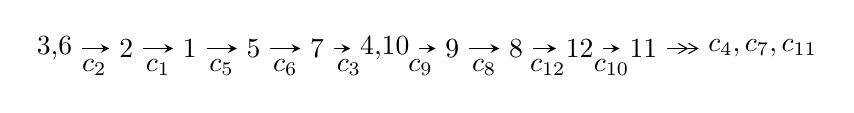
\begin{tikzpicture}[x=23pt, y=7pt]
	% node
	\node (A0) at (-1/8, 0) {3,6};
	\node (A1) at (1, 0) {2};
	\node (A2) at (2, 0) {1};
	\node (A3) at (3, 0) {5};
	\node (A4) at (4, 0) {7};
	\node (A5) at (81/16, 0) {4,10};
	\node (A6) at (49/8, 0) {9};
	\node (A7) at (57/8, 0) {8};
	\node (A8) at (65/8, 0) {12};
	\node (A9) at (73/8, 0) {11};
	\node (C1) at (1/2, -1) {$c_{2}$};
	\node (C2) at (3/2, -1) {$c_{1}$};
	\node (C3) at (5/2, -1) {$c_{5}$};
	\node (C4) at (7/2, -1) {$c_{6}$};
	\node (C5) at (9/2, -1) {$c_{3}$};
	\node (C6) at (45/8, -1) {$c_{9}$};
	\node (C7) at (53/8, -1) {$c_{8}$};
	\node (C8) at (61/8, -1) {$c_{12}$};
	\node (C9) at (69/8, -1) {$c_{10}$};
	\node (A10) at (11, 0) {$c_{4},c_{7},c_{11}$};

	% edge
	\draw[->,>=stealth]	
	(A0) edge (A1) (A1) edge (A2) (A2) edge (A3) (A3) edge (A4) (A4) edge (A5) (A5) edge (A6) (A6) edge (A7) (A7) edge (A8) (A8) edge (A9) ;
	\draw[->>,>={angle 60}]	
	(A9) edge (A10);
\end{tikzpicture} \\ 

\end{tabular} \\

\footnotetext{
The image of knot diagram is generated by the software ``\textbf{Draw programme}" developed by Andrew Bartholomew(\url{http://www.layer8.co.uk/maths/draw/index.htm\#Running-draw}), where we modified some parts for our purpose(\url{https://github.com/CATsTAILs/LinksPainter}).
}\phantom \\ \newline 
\centering \textbf{Ideals for irreducible components\footnotemark of $X_{\text{par}}$} 
 
\begin{align*}
I^u_{1}&=\langle 
13 u^{74}-40 u^{73}+\cdots+2 b+9,\;15 u^{74}-62 u^{73}+\cdots+4 a+33,\;u^{75}-4 u^{74}+\cdots+2 u-1\rangle \\
I^u_{2}&=\langle 
b,\;a^2- a u+2 u^2+3 u+2,\;u^3+u^2-1\rangle \\
I^u_{3}&=\langle 
b,\;a+1,\;u^6- u^5+2 u^2-2 u+1\rangle \\
I^u_{4}&=\langle 
b,\;a+1,\;u+1\rangle \\
I^u_{5}&=\langle 
b,\;a-1,\;u^3+u^2-1\rangle \\
\\
\end{align*}
\raggedright * 5 irreducible components of $\dim_{\mathbb{C}}=0$, with total 91 representations.\\
\footnotetext{All coefficients of polynomials are rational numbers. But the coefficients are sometimes approximated in decimal forms when there is not enough margin.}
\newpage
\renewcommand{\arraystretch}{1}
\centering \section*{I. $I^u_{1}= \langle 13 u^{74}-40 u^{73}+\cdots+2 b+9,\;15 u^{74}-62 u^{73}+\cdots+4 a+33,\;u^{75}-4 u^{74}+\cdots+2 u-1 \rangle$}
\flushleft \textbf{(i) Arc colorings}\\
\begin{tabular}{m{7pt} m{180pt} m{7pt} m{180pt} }
\flushright $a_{3}=$&$\begin{pmatrix}1\\0\end{pmatrix}$ \\
\flushright $a_{6}=$&$\begin{pmatrix}0\\u\end{pmatrix}$ \\
\flushright $a_{2}=$&$\begin{pmatrix}1\\- u^2\end{pmatrix}$ \\
\flushright $a_{1}=$&$\begin{pmatrix}- u^2+1\\- u^2\end{pmatrix}$ \\
\flushright $a_{5}=$&$\begin{pmatrix}u\\- u^3+u\end{pmatrix}$ \\
\flushright $a_{7}=$&$\begin{pmatrix}- u^3\\u^5- u^3+u\end{pmatrix}$ \\
\flushright $a_{4}=$&$\begin{pmatrix}- u^8+u^6- u^4+1\\u^{10}-2 u^8+3 u^6-2 u^4+u^2\end{pmatrix}$ \\
\flushright $a_{10}=$&$\begin{pmatrix}-3.75000 u^{74}+15.5000 u^{73}+\cdots+10.2500 u-8.25000\\-\frac{13}{2} u^{74}+20 u^{73}+\cdots+\frac{17}{2} u-\frac{9}{2}\end{pmatrix}$ \\
\flushright $a_{9}=$&$\begin{pmatrix}-8 u^{74}+\frac{115}{4} u^{73}+\cdots+\frac{57}{4} u-\frac{41}{4}\\-\frac{17}{2} u^{74}+\frac{97}{4} u^{73}+\cdots+\frac{43}{4} u-\frac{9}{2}\end{pmatrix}$ \\
\flushright $a_{8}=$&$\begin{pmatrix}4 u^{74}-\frac{67}{4} u^{73}+\cdots-\frac{17}{4} u+\frac{17}{4}\\\frac{9}{2} u^{74}-\frac{65}{4} u^{73}+\cdots-\frac{19}{4} u+\frac{9}{2}\end{pmatrix}$ \\
\flushright $a_{12}=$&$\begin{pmatrix}-\frac{1}{4} u^{72}+\frac{3}{4} u^{71}+\cdots+\frac{7}{2} u+\frac{1}{4}\\u^{19}-3 u^{17}+\cdots-4 u^2+u\end{pmatrix}$ \\
\flushright $a_{11}=$&$\begin{pmatrix}\frac{9}{4} u^{73}-\frac{23}{4} u^{72}+\cdots+\frac{21}{2} u^2-\frac{35}{4} u\\-\frac{7}{2} u^{74}+\frac{51}{4} u^{73}+\cdots+\frac{9}{4} u-\frac{7}{2}\end{pmatrix}$\\&\end{tabular}
\flushleft \textbf{(ii) Obstruction class $= -1$}\\~\\
\flushleft \textbf{(iii) Cusp Shapes $= \frac{31}{4} u^{74}-\frac{3}{2} u^{73}+\cdots+\frac{3}{4} u-\frac{37}{2}$}\\~\\
\newpage\renewcommand{\arraystretch}{1}
\flushleft \textbf{(iv) u-Polynomials at the component}\newline \\
\begin{tabular}{m{50pt}|m{274pt}}
Crossings & \hspace{64pt}u-Polynomials at each crossing \\
\hline $$\begin{aligned}c_{1},c_{6}\end{aligned}$$&$\begin{aligned}
&u^{75}+26 u^{74}+\cdots-6 u+1
\end{aligned}$\\
\hline $$\begin{aligned}c_{2},c_{5}\end{aligned}$$&$\begin{aligned}
&u^{75}+4 u^{74}+\cdots+2 u+1
\end{aligned}$\\
\hline $$\begin{aligned}c_{3}\end{aligned}$$&$\begin{aligned}
&u^{75}-4 u^{74}+\cdots+3428 u+673
\end{aligned}$\\
\hline $$\begin{aligned}c_{4},c_{8}\end{aligned}$$&$\begin{aligned}
&u^{75}-6 u^{74}+\cdots-2048 u+512
\end{aligned}$\\
\hline $$\begin{aligned}c_{7},c_{11}\end{aligned}$$&$\begin{aligned}
&u^{75}-4 u^{74}+\cdots+2 u+1
\end{aligned}$\\
\hline $$\begin{aligned}c_{9},c_{10},c_{12}\end{aligned}$$&$\begin{aligned}
&u^{75}-18 u^{74}+\cdots+42 u-1
\end{aligned}$\\
\hline
\end{tabular}\\~\\
\newpage\renewcommand{\arraystretch}{1}
\flushleft \textbf{(v) Riley Polynomials at the component}\newline \\
\begin{tabular}{m{50pt}|m{274pt}}
Crossings & \hspace{64pt}Riley Polynomials at each crossing \\
\hline $$\begin{aligned}c_{1},c_{6}\end{aligned}$$&$\begin{aligned}
&y^{75}+50 y^{74}+\cdots+338 y-1
\end{aligned}$\\
\hline $$\begin{aligned}c_{2},c_{5}\end{aligned}$$&$\begin{aligned}
&y^{75}-26 y^{74}+\cdots-6 y-1
\end{aligned}$\\
\hline $$\begin{aligned}c_{3}\end{aligned}$$&$\begin{aligned}
&y^{75}-34 y^{74}+\cdots+20450382 y-452929
\end{aligned}$\\
\hline $$\begin{aligned}c_{4},c_{8}\end{aligned}$$&$\begin{aligned}
&y^{75}-42 y^{74}+\cdots+2228224 y-262144
\end{aligned}$\\
\hline $$\begin{aligned}c_{7},c_{11}\end{aligned}$$&$\begin{aligned}
&y^{75}-18 y^{74}+\cdots+42 y-1
\end{aligned}$\\
\hline $$\begin{aligned}c_{9},c_{10},c_{12}\end{aligned}$$&$\begin{aligned}
&y^{75}+82 y^{74}+\cdots+898 y-1
\end{aligned}$\\
\hline
\end{tabular}\\~\\
\newpage\flushleft \textbf{(vi) Complex Volumes and Cusp Shapes}
$$\begin{array}{c|c|c}  
\text{Solutions to }I^u_{1}& \I (\text{vol} + \sqrt{-1}CS) & \text{Cusp shape}\\
 \hline 
\begin{aligned}
u &= \phantom{-}0.701208 + 0.720685 I \\
a &= \phantom{-}0.271979 - 0.246067 I \\
b &= -0.579346 - 0.610917 I\end{aligned}
 & \phantom{-}3.38308 - 0.01973 I & \phantom{-0.000000 } 0 \\ \hline\begin{aligned}
u &= \phantom{-}0.701208 - 0.720685 I \\
a &= \phantom{-}0.271979 + 0.246067 I \\
b &= -0.579346 + 0.610917 I\end{aligned}
 & \phantom{-}3.38308 + 0.01973 I & \phantom{-0.000000 } 0 \\ \hline\begin{aligned}
u &= \phantom{-}0.627949 + 0.758720 I \\
a &= -0.575313 + 1.104250 I \\
b &= \phantom{-}0.241056 + 1.106360 I\end{aligned}
 & -0.61116 + 1.98602 I & \phantom{-0.000000 } 0 \\ \hline\begin{aligned}
u &= \phantom{-}0.627949 - 0.758720 I \\
a &= -0.575313 - 1.104250 I \\
b &= \phantom{-}0.241056 - 1.106360 I\end{aligned}
 & -0.61116 - 1.98602 I & \phantom{-0.000000 } 0 \\ \hline\begin{aligned}
u &= \phantom{-}0.797274 + 0.636830 I \\
a &= \phantom{-}1.023330 + 0.109881 I \\
b &= -0.383426 - 0.229792 I\end{aligned}
 & -1.24153 - 4.89896 I & \phantom{-0.000000 } 0 \\ \hline\begin{aligned}
u &= \phantom{-}0.797274 - 0.636830 I \\
a &= \phantom{-}1.023330 - 0.109881 I \\
b &= -0.383426 + 0.229792 I\end{aligned}
 & -1.24153 + 4.89896 I & \phantom{-0.000000 } 0 \\ \hline\begin{aligned}
u &= \phantom{-}0.663944 + 0.796185 I \\
a &= -0.228762 - 1.369140 I \\
b &= -0.75083 - 1.34544 I\end{aligned}
 & \phantom{-}1.75797 + 5.85887 I & \phantom{-0.000000 } 0 \\ \hline\begin{aligned}
u &= \phantom{-}0.663944 - 0.796185 I \\
a &= -0.228762 + 1.369140 I \\
b &= -0.75083 + 1.34544 I\end{aligned}
 & \phantom{-}1.75797 - 5.85887 I & \phantom{-0.000000 } 0 \\ \hline\begin{aligned}
u &= \phantom{-}0.809697 + 0.500286 I \\
a &= -1.101780 + 0.206259 I \\
b &= \phantom{-}0.331049 + 0.357019 I\end{aligned}
 & -1.80504 + 0.21281 I & \phantom{-0.000000 } 0 \\ \hline\begin{aligned}
u &= \phantom{-}0.809697 - 0.500286 I \\
a &= -1.101780 - 0.206259 I \\
b &= \phantom{-}0.331049 - 0.357019 I\end{aligned}
 & -1.80504 - 0.21281 I & \phantom{-0.000000 } 0\\
 \hline 
 \end{array}$$\newpage$$\begin{array}{c|c|c}  
\text{Solutions to }I^u_{1}& \I (\text{vol} + \sqrt{-1}CS) & \text{Cusp shape}\\
 \hline 
\begin{aligned}
u &= -0.746204 + 0.738382 I \\
a &= -1.06503 + 1.47927 I \\
b &= -1.32562 + 0.86777 I\end{aligned}
 & \phantom{-}3.84873 - 0.66860 I & \phantom{-0.000000 } 0 \\ \hline\begin{aligned}
u &= -0.746204 - 0.738382 I \\
a &= -1.06503 - 1.47927 I \\
b &= -1.32562 - 0.86777 I\end{aligned}
 & \phantom{-}3.84873 + 0.66860 I & \phantom{-0.000000 } 0 \\ \hline\begin{aligned}
u &= -0.628281 + 0.711921 I \\
a &= -1.12592 + 3.33671 I \\
b &= -1.41795 + 1.94907 I\end{aligned}
 & -3.10213 - 3.84461 I & \phantom{-0.000000 } 0 \\ \hline\begin{aligned}
u &= -0.628281 - 0.711921 I \\
a &= -1.12592 - 3.33671 I \\
b &= -1.41795 - 1.94907 I\end{aligned}
 & -3.10213 + 3.84461 I & \phantom{-0.000000 } 0 \\ \hline\begin{aligned}
u &= \phantom{-}0.627365 + 0.846180 I \\
a &= -0.14858 + 2.83753 I \\
b &= \phantom{-}0.46848 + 2.31286 I\end{aligned}
 & -6.70348 + 3.72129 I & \phantom{-0.000000 } 0 \\ \hline\begin{aligned}
u &= \phantom{-}0.627365 - 0.846180 I \\
a &= -0.14858 - 2.83753 I \\
b &= \phantom{-}0.46848 - 2.31286 I\end{aligned}
 & -6.70348 - 3.72129 I & \phantom{-0.000000 } 0 \\ \hline\begin{aligned}
u &= -1.051230 + 0.097083 I \\
a &= -0.311756 - 0.810124 I \\
b &= \phantom{-}0.066769 + 1.046900 I\end{aligned}
 & -4.37588 + 5.64662 I & \phantom{-0.000000 } 0 \\ \hline\begin{aligned}
u &= -1.051230 - 0.097083 I \\
a &= -0.311756 + 0.810124 I \\
b &= \phantom{-}0.066769 - 1.046900 I\end{aligned}
 & -4.37588 - 5.64662 I & \phantom{-0.000000 } 0 \\ \hline\begin{aligned}
u &= -0.812700 + 0.676974 I \\
a &= -0.188335 - 1.356770 I \\
b &= \phantom{-}0.615066 - 1.037800 I\end{aligned}
 & \phantom{-}2.12142 + 2.26372 I & \phantom{-0.000000 } 0 \\ \hline\begin{aligned}
u &= -0.812700 - 0.676974 I \\
a &= -0.188335 + 1.356770 I \\
b &= \phantom{-}0.615066 + 1.037800 I\end{aligned}
 & \phantom{-}2.12142 - 2.26372 I & \phantom{-0.000000 } 0\\
 \hline 
 \end{array}$$\newpage$$\begin{array}{c|c|c}  
\text{Solutions to }I^u_{1}& \I (\text{vol} + \sqrt{-1}CS) & \text{Cusp shape}\\
 \hline 
\begin{aligned}
u &= \phantom{-}1.060630 + 0.009927 I \\
a &= \phantom{-}0.004661 + 1.039530 I \\
b &= \phantom{-}0.20878 - 3.03992 I\end{aligned}
 & -8.40746 - 3.15444 I & \phantom{-0.000000 } 0 \\ \hline\begin{aligned}
u &= \phantom{-}1.060630 - 0.009927 I \\
a &= \phantom{-}0.004661 - 1.039530 I \\
b &= \phantom{-}0.20878 + 3.03992 I\end{aligned}
 & -8.40746 + 3.15444 I & \phantom{-0.000000 } 0 \\ \hline\begin{aligned}
u &= \phantom{-}0.638608 + 0.850784 I \\
a &= -0.21667 - 2.89559 I \\
b &= -0.71638 - 2.35011 I\end{aligned}
 & -6.21701 + 10.10530 I & \phantom{-0.000000 } 0 \\ \hline\begin{aligned}
u &= \phantom{-}0.638608 - 0.850784 I \\
a &= -0.21667 + 2.89559 I \\
b &= -0.71638 + 2.35011 I\end{aligned}
 & -6.21701 - 10.10530 I & \phantom{-0.000000 } 0 \\ \hline\begin{aligned}
u &= \phantom{-}0.932954 + 0.071441 I \\
a &= -0.193432 + 0.886433 I \\
b &= \phantom{-}0.625448 - 1.099660 I\end{aligned}
 & -1.44111 - 1.48666 I & -6.77628 + 4.80712 I \\ \hline\begin{aligned}
u &= \phantom{-}0.932954 - 0.071441 I \\
a &= -0.193432 - 0.886433 I \\
b &= \phantom{-}0.625448 + 1.099660 I\end{aligned}
 & -1.44111 + 1.48666 I & -6.77628 - 4.80712 I \\ \hline\begin{aligned}
u &= -1.071330 + 0.046708 I \\
a &= \phantom{-}0.314563 + 0.332337 I \\
b &= \phantom{-}0.600863 - 0.674517 I\end{aligned}
 & -6.34634 + 1.36308 I & \phantom{-0.000000 } 0 \\ \hline\begin{aligned}
u &= -1.071330 - 0.046708 I \\
a &= \phantom{-}0.314563 - 0.332337 I \\
b &= \phantom{-}0.600863 + 0.674517 I\end{aligned}
 & -6.34634 - 1.36308 I & \phantom{-0.000000 } 0 \\ \hline\begin{aligned}
u &= -0.619084 + 0.677506 I \\
a &= \phantom{-}0.66146 - 3.38346 I \\
b &= \phantom{-}1.12813 - 1.94943 I\end{aligned}
 & -3.32990 + 2.33530 I & -2.00000 - 3.24885 I \\ \hline\begin{aligned}
u &= -0.619084 - 0.677506 I \\
a &= \phantom{-}0.66146 + 3.38346 I \\
b &= \phantom{-}1.12813 + 1.94943 I\end{aligned}
 & -3.32990 - 2.33530 I & -2.00000 + 3.24885 I\\
 \hline 
 \end{array}$$\newpage$$\begin{array}{c|c|c}  
\text{Solutions to }I^u_{1}& \I (\text{vol} + \sqrt{-1}CS) & \text{Cusp shape}\\
 \hline 
\begin{aligned}
u &= -0.911078 + 0.665908 I \\
a &= -1.46979 - 0.72717 I \\
b &= -0.265473 - 1.359370 I\end{aligned}
 & \phantom{-}1.81337 + 2.92907 I & \phantom{-0.000000 } 0 \\ \hline\begin{aligned}
u &= -0.911078 - 0.665908 I \\
a &= -1.46979 + 0.72717 I \\
b &= -0.265473 + 1.359370 I\end{aligned}
 & \phantom{-}1.81337 - 2.92907 I & \phantom{-0.000000 } 0 \\ \hline\begin{aligned}
u &= -1.126690 + 0.126000 I \\
a &= \phantom{-}0.492982 - 0.635491 I \\
b &= -0.24597 + 2.58837 I\end{aligned}
 & -12.9589 + 9.4189 I & \phantom{-0.000000 } 0 \\ \hline\begin{aligned}
u &= -1.126690 - 0.126000 I \\
a &= \phantom{-}0.492982 + 0.635491 I \\
b &= -0.24597 - 2.58837 I\end{aligned}
 & -12.9589 - 9.4189 I & \phantom{-0.000000 } 0 \\ \hline\begin{aligned}
u &= -1.129400 + 0.113156 I \\
a &= -0.413730 + 0.513608 I \\
b &= \phantom{-}0.57600 - 2.46752 I\end{aligned}
 & -13.35070 + 2.93555 I & \phantom{-0.000000 } 0 \\ \hline\begin{aligned}
u &= -1.129400 - 0.113156 I \\
a &= -0.413730 - 0.513608 I \\
b &= \phantom{-}0.57600 + 2.46752 I\end{aligned}
 & -13.35070 - 2.93555 I & \phantom{-0.000000 } 0 \\ \hline\begin{aligned}
u &= -0.831632 + 0.781731 I \\
a &= -0.405448 + 0.090942 I \\
b &= -0.717939 + 0.023903 I\end{aligned}
 & \phantom{-}4.49518 + 3.61543 I & \phantom{-0.000000 } 0 \\ \hline\begin{aligned}
u &= -0.831632 - 0.781731 I \\
a &= -0.405448 - 0.090942 I \\
b &= -0.717939 - 0.023903 I\end{aligned}
 & \phantom{-}4.49518 - 3.61543 I & \phantom{-0.000000 } 0 \\ \hline\begin{aligned}
u &= \phantom{-}1.054410 + 0.511172 I \\
a &= -2.54504 - 0.47126 I \\
b &= -1.17837 + 1.55125 I\end{aligned}
 & -10.59020 + 2.33640 I & \phantom{-0.000000 } 0 \\ \hline\begin{aligned}
u &= \phantom{-}1.054410 - 0.511172 I \\
a &= -2.54504 + 0.47126 I \\
b &= -1.17837 - 1.55125 I\end{aligned}
 & -10.59020 - 2.33640 I & \phantom{-0.000000 } 0\\
 \hline 
 \end{array}$$\newpage$$\begin{array}{c|c|c}  
\text{Solutions to }I^u_{1}& \I (\text{vol} + \sqrt{-1}CS) & \text{Cusp shape}\\
 \hline 
\begin{aligned}
u &= \phantom{-}0.996108 + 0.618806 I \\
a &= \phantom{-}0.657831 + 0.669598 I \\
b &= \phantom{-}0.536812 + 0.383150 I\end{aligned}
 & -2.90368 - 4.76352 I & \phantom{-0.000000 } 0 \\ \hline\begin{aligned}
u &= \phantom{-}0.996108 - 0.618806 I \\
a &= \phantom{-}0.657831 - 0.669598 I \\
b &= \phantom{-}0.536812 - 0.383150 I\end{aligned}
 & -2.90368 + 4.76352 I & \phantom{-0.000000 } 0 \\ \hline\begin{aligned}
u &= \phantom{-}1.056010 + 0.527223 I \\
a &= \phantom{-}2.46210 + 0.75720 I \\
b &= \phantom{-}1.41911 - 1.29282 I\end{aligned}
 & -10.79530 - 4.15159 I & \phantom{-0.000000 } 0 \\ \hline\begin{aligned}
u &= \phantom{-}1.056010 - 0.527223 I \\
a &= \phantom{-}2.46210 - 0.75720 I \\
b &= \phantom{-}1.41911 + 1.29282 I\end{aligned}
 & -10.79530 + 4.15159 I & \phantom{-0.000000 } 0 \\ \hline\begin{aligned}
u &= -0.959804 + 0.703274 I \\
a &= \phantom{-}2.06554 - 0.50300 I \\
b &= \phantom{-}1.26162 + 1.12681 I\end{aligned}
 & \phantom{-}3.20109 + 6.17050 I & \phantom{-0.000000 } 0 \\ \hline\begin{aligned}
u &= -0.959804 - 0.703274 I \\
a &= \phantom{-}2.06554 + 0.50300 I \\
b &= \phantom{-}1.26162 - 1.12681 I\end{aligned}
 & \phantom{-}3.20109 - 6.17050 I & \phantom{-0.000000 } 0 \\ \hline\begin{aligned}
u &= -0.915099 + 0.761150 I \\
a &= \phantom{-}0.276923 - 0.700562 I \\
b &= \phantom{-}0.598686 + 0.067274 I\end{aligned}
 & \phantom{-}4.24134 + 2.19377 I & \phantom{-0.000000 } 0 \\ \hline\begin{aligned}
u &= -0.915099 - 0.761150 I \\
a &= \phantom{-}0.276923 + 0.700562 I \\
b &= \phantom{-}0.598686 - 0.067274 I\end{aligned}
 & \phantom{-}4.24134 - 2.19377 I & \phantom{-0.000000 } 0 \\ \hline\begin{aligned}
u &= \phantom{-}0.292739 + 0.750663 I \\
a &= -1.32844 - 2.03101 I \\
b &= -0.57813 - 1.46945 I\end{aligned}
 & -8.54207 - 0.47640 I & -5.31082 + 0.38811 I \\ \hline\begin{aligned}
u &= \phantom{-}0.292739 - 0.750663 I \\
a &= -1.32844 + 2.03101 I \\
b &= -0.57813 + 1.46945 I\end{aligned}
 & -8.54207 + 0.47640 I & -5.31082 - 0.38811 I\\
 \hline 
 \end{array}$$\newpage$$\begin{array}{c|c|c}  
\text{Solutions to }I^u_{1}& \I (\text{vol} + \sqrt{-1}CS) & \text{Cusp shape}\\
 \hline 
\begin{aligned}
u &= \phantom{-}0.983291 + 0.679379 I \\
a &= \phantom{-}0.326271 + 0.217290 I \\
b &= \phantom{-}0.269460 - 0.782508 I\end{aligned}
 & \phantom{-}2.52825 - 5.35908 I & \phantom{-0.000000 } 0 \\ \hline\begin{aligned}
u &= \phantom{-}0.983291 - 0.679379 I \\
a &= \phantom{-}0.326271 - 0.217290 I \\
b &= \phantom{-}0.269460 + 0.782508 I\end{aligned}
 & \phantom{-}2.52825 + 5.35908 I & \phantom{-0.000000 } 0 \\ \hline\begin{aligned}
u &= -1.005430 + 0.652614 I \\
a &= -3.71899 - 0.62315 I \\
b &= -1.43602 - 2.72402 I\end{aligned}
 & -4.45485 + 2.85370 I & \phantom{-0.000000 } 0 \\ \hline\begin{aligned}
u &= -1.005430 - 0.652614 I \\
a &= -3.71899 + 0.62315 I \\
b &= -1.43602 + 2.72402 I\end{aligned}
 & -4.45485 - 2.85370 I & \phantom{-0.000000 } 0 \\ \hline\begin{aligned}
u &= \phantom{-}0.267962 + 0.749469 I \\
a &= \phantom{-}0.96458 + 2.24772 I \\
b &= \phantom{-}0.33863 + 1.65527 I\end{aligned}
 & -8.25339 - 6.87058 I & -4.66942 + 5.31459 I \\ \hline\begin{aligned}
u &= \phantom{-}0.267962 - 0.749469 I \\
a &= \phantom{-}0.96458 - 2.24772 I \\
b &= \phantom{-}0.33863 - 1.65527 I\end{aligned}
 & -8.25339 + 6.87058 I & -4.66942 - 5.31459 I \\ \hline\begin{aligned}
u &= -1.009510 + 0.664597 I \\
a &= \phantom{-}3.84862 + 0.23046 I \\
b &= \phantom{-}1.76093 + 2.58718 I\end{aligned}
 & -4.22333 + 9.15433 I & \phantom{-0.000000 } 0 \\ \hline\begin{aligned}
u &= -1.009510 - 0.664597 I \\
a &= \phantom{-}3.84862 - 0.23046 I \\
b &= \phantom{-}1.76093 - 2.58718 I\end{aligned}
 & -4.22333 - 9.15433 I & \phantom{-0.000000 } 0 \\ \hline\begin{aligned}
u &= -0.884174 + 0.827701 I \\
a &= \phantom{-}0.858746 - 0.332274 I \\
b &= -0.020477 - 0.186379 I\end{aligned}
 & -1.61016 + 6.14153 I & \phantom{-0.000000 } 0 \\ \hline\begin{aligned}
u &= -0.884174 - 0.827701 I \\
a &= \phantom{-}0.858746 + 0.332274 I \\
b &= -0.020477 + 0.186379 I\end{aligned}
 & -1.61016 - 6.14153 I & \phantom{-0.000000 } 0\\
 \hline 
 \end{array}$$\newpage$$\begin{array}{c|c|c}  
\text{Solutions to }I^u_{1}& \I (\text{vol} + \sqrt{-1}CS) & \text{Cusp shape}\\
 \hline 
\begin{aligned}
u &= \phantom{-}1.020350 + 0.680346 I \\
a &= -1.026190 + 0.714206 I \\
b &= -0.02211 + 1.47609 I\end{aligned}
 & -1.77547 - 7.46274 I & \phantom{-0.000000 } 0 \\ \hline\begin{aligned}
u &= \phantom{-}1.020350 - 0.680346 I \\
a &= -1.026190 - 0.714206 I \\
b &= -0.02211 - 1.47609 I\end{aligned}
 & -1.77547 + 7.46274 I & \phantom{-0.000000 } 0 \\ \hline\begin{aligned}
u &= \phantom{-}1.018070 + 0.704584 I \\
a &= \phantom{-}1.78244 - 0.14154 I \\
b &= \phantom{-}0.63403 - 1.61362 I\end{aligned}
 & \phantom{-}0.68795 - 11.52010 I & \phantom{-0.000000 } 0 \\ \hline\begin{aligned}
u &= \phantom{-}1.018070 - 0.704584 I \\
a &= \phantom{-}1.78244 + 0.14154 I \\
b &= \phantom{-}0.63403 + 1.61362 I\end{aligned}
 & \phantom{-}0.68795 + 11.52010 I & \phantom{-0.000000 } 0 \\ \hline\begin{aligned}
u &= \phantom{-}1.050580 + 0.711144 I \\
a &= -2.84228 + 1.32579 I \\
b &= -0.58040 + 2.70950 I\end{aligned}
 & -7.99110 - 9.53376 I & \phantom{-0.000000 } 0 \\ \hline\begin{aligned}
u &= \phantom{-}1.050580 - 0.711144 I \\
a &= -2.84228 - 1.32579 I \\
b &= -0.58040 - 2.70950 I\end{aligned}
 & -7.99110 + 9.53376 I & \phantom{-0.000000 } 0 \\ \hline\begin{aligned}
u &= \phantom{-}1.048440 + 0.717583 I \\
a &= \phantom{-}3.10399 - 1.06144 I \\
b &= \phantom{-}0.84917 - 2.69538 I\end{aligned}
 & -7.4670 - 15.9552 I & \phantom{-0.000000 } 0 \\ \hline\begin{aligned}
u &= \phantom{-}1.048440 - 0.717583 I \\
a &= \phantom{-}3.10399 + 1.06144 I \\
b &= \phantom{-}0.84917 + 2.69538 I\end{aligned}
 & -7.4670 + 15.9552 I & \phantom{-0.000000 } 0 \\ \hline\begin{aligned}
u &= \phantom{-}0.649139\phantom{ +0.000000I} \\
a &= -0.546045\phantom{ +0.000000I} \\
b &= \phantom{-}0.341478\phantom{ +0.000000I}\end{aligned}
 & -0.884135\phantom{ +0.000000I} & -11.8620\phantom{ +0.000000I} \\ \hline\begin{aligned}
u &= \phantom{-}0.233494 + 0.573241 I \\
a &= \phantom{-}0.058819 + 0.473224 I \\
b &= -0.477292 + 0.578592 I\end{aligned}
 & -0.29565 - 3.74527 I & -0.52170 + 7.33925 I\\
 \hline 
 \end{array}$$\newpage$$\begin{array}{c|c|c}  
\text{Solutions to }I^u_{1}& \I (\text{vol} + \sqrt{-1}CS) & \text{Cusp shape}\\
 \hline 
\begin{aligned}
u &= \phantom{-}0.233494 - 0.573241 I \\
a &= \phantom{-}0.058819 - 0.473224 I \\
b &= -0.477292 - 0.578592 I\end{aligned}
 & -0.29565 + 3.74527 I & -0.52170 - 7.33925 I \\ \hline\begin{aligned}
u &= -0.475208 + 0.051931 I \\
a &= -0.18074 - 3.75063 I \\
b &= \phantom{-}0.015921 - 0.686883 I\end{aligned}
 & -3.67022 + 2.91113 I & \phantom{-}3.44925 - 3.93604 I \\ \hline\begin{aligned}
u &= -0.475208 - 0.051931 I \\
a &= -0.18074 + 3.75063 I \\
b &= \phantom{-}0.015921 + 0.686883 I\end{aligned}
 & -3.67022 - 2.91113 I & \phantom{-}3.44925 + 3.93604 I \\ \hline\begin{aligned}
u &= -0.028799 + 0.274080 I \\
a &= \phantom{-}0.18442 - 1.93169 I \\
b &= -0.520994 - 0.325782 I\end{aligned}
 & \phantom{-}1.326270 + 0.342139 I & \phantom{-}6.30252 - 0.67770 I \\ \hline\begin{aligned}
u &= -0.028799 - 0.274080 I \\
a &= \phantom{-}0.18442 + 1.93169 I \\
b &= -0.520994 + 0.325782 I\end{aligned}
 & \phantom{-}1.326270 - 0.342139 I & \phantom{-}6.30252 + 0.67770 I\\
 \hline 
 \end{array}$$\newpage\newpage\renewcommand{\arraystretch}{1}
\centering \section*{II. $I^u_{2}= \langle b,\;a^2- a u+2 u^2+3 u+2,\;u^3+u^2-1 \rangle$}
\flushleft \textbf{(i) Arc colorings}\\
\begin{tabular}{m{7pt} m{180pt} m{7pt} m{180pt} }
\flushright $a_{3}=$&$\begin{pmatrix}1\\0\end{pmatrix}$ \\
\flushright $a_{6}=$&$\begin{pmatrix}0\\u\end{pmatrix}$ \\
\flushright $a_{2}=$&$\begin{pmatrix}1\\- u^2\end{pmatrix}$ \\
\flushright $a_{1}=$&$\begin{pmatrix}- u^2+1\\- u^2\end{pmatrix}$ \\
\flushright $a_{5}=$&$\begin{pmatrix}u\\u^2+u-1\end{pmatrix}$ \\
\flushright $a_{7}=$&$\begin{pmatrix}u^2-1\\u^2\end{pmatrix}$ \\
\flushright $a_{4}=$&$\begin{pmatrix}u\\u^2+u-1\end{pmatrix}$ \\
\flushright $a_{10}=$&$\begin{pmatrix}a\\0\end{pmatrix}$ \\
\flushright $a_{9}=$&$\begin{pmatrix}a u\\u^2 a+a u- a\end{pmatrix}$ \\
\flushright $a_{8}=$&$\begin{pmatrix}a u\\u^2 a+a u- a\end{pmatrix}$ \\
\flushright $a_{12}=$&$\begin{pmatrix}- u^2 a-2 u^2+a-2 u\\- u^2\end{pmatrix}$ \\
\flushright $a_{11}=$&$\begin{pmatrix}- u^2 a- a u- u^2+a- u\\- u^2 a- a u+a\end{pmatrix}$\\&\end{tabular}
\flushleft \textbf{(ii) Obstruction class $= 1$}\\~\\
\flushleft \textbf{(iii) Cusp Shapes $= - u^2 a- u^2-8 u-7$}\\~\\
\newpage\renewcommand{\arraystretch}{1}
\flushleft \textbf{(iv) u-Polynomials at the component}\newline \\
\begin{tabular}{m{50pt}|m{274pt}}
Crossings & \hspace{64pt}u-Polynomials at each crossing \\
\hline $$\begin{aligned}c_{1},c_{3},c_{12}\end{aligned}$$&$\begin{aligned}
&(u^3- u^2+2 u-1)^2
\end{aligned}$\\
\hline $$\begin{aligned}c_{2},c_{11}\end{aligned}$$&$\begin{aligned}
&(u^3+u^2-1)^2
\end{aligned}$\\
\hline $$\begin{aligned}c_{4},c_{8}\end{aligned}$$&$\begin{aligned}
&u^6
\end{aligned}$\\
\hline $$\begin{aligned}c_{5},c_{7}\end{aligned}$$&$\begin{aligned}
&(u^3- u^2+1)^2
\end{aligned}$\\
\hline $$\begin{aligned}c_{6},c_{9},c_{10}\end{aligned}$$&$\begin{aligned}
&(u^3+u^2+2 u+1)^2
\end{aligned}$\\
\hline
\end{tabular}\\~\\
\newpage\renewcommand{\arraystretch}{1}
\flushleft \textbf{(v) Riley Polynomials at the component}\newline \\
\begin{tabular}{m{50pt}|m{274pt}}
Crossings & \hspace{64pt}Riley Polynomials at each crossing \\
\hline $$\begin{aligned}c_{1},c_{3},c_{6}\\c_{9},c_{10},c_{12}\end{aligned}$$&$\begin{aligned}
&(y^3+3 y^2+2 y-1)^2
\end{aligned}$\\
\hline $$\begin{aligned}c_{2},c_{5},c_{7}\\c_{11}\end{aligned}$$&$\begin{aligned}
&(y^3- y^2+2 y-1)^2
\end{aligned}$\\
\hline $$\begin{aligned}c_{4},c_{8}\end{aligned}$$&$\begin{aligned}
&y^6
\end{aligned}$\\
\hline
\end{tabular}\\~\\
\newpage\flushleft \textbf{(vi) Complex Volumes and Cusp Shapes}
$$\begin{array}{c|c|c}  
\text{Solutions to }I^u_{2}& \I (\text{vol} + \sqrt{-1}CS) & \text{Cusp shape}\\
 \hline 
\begin{aligned}
u &= -0.877439 + 0.744862 I \\
a &= -0.947279 + 0.320410 I \\
b &= \phantom{-0.000000 } 0\end{aligned}
 & \phantom{-0.000000 -}5.65624 I & -0.41065 - 5.95889 I \\ \hline\begin{aligned}
u &= -0.877439 + 0.744862 I \\
a &= \phantom{-}0.069840 + 0.424452 I \\
b &= \phantom{-0.000000 } 0\end{aligned}
 & \phantom{-}4.13758 + 2.82812 I & -0.76541 - 4.65175 I \\ \hline\begin{aligned}
u &= -0.877439 - 0.744862 I \\
a &= -0.947279 - 0.320410 I \\
b &= \phantom{-0.000000 } 0\end{aligned}
 & \phantom{-0.000000 } -5.65624 I & -0.41065 + 5.95889 I \\ \hline\begin{aligned}
u &= -0.877439 - 0.744862 I \\
a &= \phantom{-}0.069840 - 0.424452 I \\
b &= \phantom{-0.000000 } 0\end{aligned}
 & \phantom{-}4.13758 - 2.82812 I & -0.76541 + 4.65175 I \\ \hline\begin{aligned}
u &= \phantom{-}0.754878\phantom{ +0.000000I} \\
a &= \phantom{-}0.37744 + 2.29387 I \\
b &= \phantom{-0.000000 } 0\end{aligned}
 & -4.13758 + 2.82812 I & -13.82394 - 1.30714 I \\ \hline\begin{aligned}
u &= \phantom{-}0.754878\phantom{ +0.000000I} \\
a &= \phantom{-}0.37744 - 2.29387 I \\
b &= \phantom{-0.000000 } 0\end{aligned}
 & -4.13758 - 2.82812 I & -13.82394 + 1.30714 I\\
 \hline 
 \end{array}$$\newpage\newpage\renewcommand{\arraystretch}{1}
\centering \section*{III. $I^u_{3}= \langle b,\;a+1,\;u^6- u^5+2 u^2-2 u+1 \rangle$}
\flushleft \textbf{(i) Arc colorings}\\
\begin{tabular}{m{7pt} m{180pt} m{7pt} m{180pt} }
\flushright $a_{3}=$&$\begin{pmatrix}1\\0\end{pmatrix}$ \\
\flushright $a_{6}=$&$\begin{pmatrix}0\\u\end{pmatrix}$ \\
\flushright $a_{2}=$&$\begin{pmatrix}1\\- u^2\end{pmatrix}$ \\
\flushright $a_{1}=$&$\begin{pmatrix}- u^2+1\\- u^2\end{pmatrix}$ \\
\flushright $a_{5}=$&$\begin{pmatrix}u\\- u^3+u\end{pmatrix}$ \\
\flushright $a_{7}=$&$\begin{pmatrix}- u^3\\u^5- u^3+u\end{pmatrix}$ \\
\flushright $a_{4}=$&$\begin{pmatrix}u^4- u^2+u+1\\u^4- u^3+u\end{pmatrix}$ \\
\flushright $a_{10}=$&$\begin{pmatrix}-1\\0\end{pmatrix}$ \\
\flushright $a_{9}=$&$\begin{pmatrix}- u^4+u^2-1\\- u^4\end{pmatrix}$ \\
\flushright $a_{8}=$&$\begin{pmatrix}u\\- u^3+u\end{pmatrix}$ \\
\flushright $a_{12}=$&$\begin{pmatrix}1\\- u^2\end{pmatrix}$ \\
\flushright $a_{11}=$&$\begin{pmatrix}- u^2-1\\u^4\end{pmatrix}$\\&\end{tabular}
\flushleft \textbf{(ii) Obstruction class $= -1$}\\~\\
\flushleft \textbf{(iii) Cusp Shapes $= -6$}\\~\\
\newpage\renewcommand{\arraystretch}{1}
\flushleft \textbf{(iv) u-Polynomials at the component}\newline \\
\begin{tabular}{m{50pt}|m{274pt}}
Crossings & \hspace{64pt}u-Polynomials at each crossing \\
\hline $$\begin{aligned}c_{1},c_{6}\end{aligned}$$&$\begin{aligned}
&u^6+u^5+4 u^4+2 u^3+4 u^2+1
\end{aligned}$\\
\hline $$\begin{aligned}c_{2},c_{5},c_{7}\\c_{11}\end{aligned}$$&$\begin{aligned}
&u^6+u^5+2 u^2+2 u+1
\end{aligned}$\\
\hline $$\begin{aligned}c_{3}\end{aligned}$$&$\begin{aligned}
&u^6+u^5+4 u^4+2 u^3-2 u^2+1
\end{aligned}$\\
\hline $$\begin{aligned}c_{4},c_{8}\end{aligned}$$&$\begin{aligned}
&(u+1)^6
\end{aligned}$\\
\hline $$\begin{aligned}c_{9},c_{10},c_{12}\end{aligned}$$&$\begin{aligned}
&u^6- u^5+4 u^4-2 u^3+4 u^2+1
\end{aligned}$\\
\hline
\end{tabular}\\~\\
\newpage\renewcommand{\arraystretch}{1}
\flushleft \textbf{(v) Riley Polynomials at the component}\newline \\
\begin{tabular}{m{50pt}|m{274pt}}
Crossings & \hspace{64pt}Riley Polynomials at each crossing \\
\hline $$\begin{aligned}c_{1},c_{6},c_{9}\\c_{10},c_{12}\end{aligned}$$&$\begin{aligned}
&y^6+7 y^5+20 y^4+30 y^3+24 y^2+8 y+1
\end{aligned}$\\
\hline $$\begin{aligned}c_{2},c_{5},c_{7}\\c_{11}\end{aligned}$$&$\begin{aligned}
&y^6- y^5+4 y^4-2 y^3+4 y^2+1
\end{aligned}$\\
\hline $$\begin{aligned}c_{3}\end{aligned}$$&$\begin{aligned}
&y^6+7 y^5+8 y^4-18 y^3+12 y^2-4 y+1
\end{aligned}$\\
\hline $$\begin{aligned}c_{4},c_{8}\end{aligned}$$&$\begin{aligned}
&(y-1)^6
\end{aligned}$\\
\hline
\end{tabular}\\~\\
\newpage\flushleft \textbf{(vi) Complex Volumes and Cusp Shapes}
$$\begin{array}{c|c|c}  
\text{Solutions to }I^u_{3}& \I (\text{vol} + \sqrt{-1}CS) & \text{Cusp shape}\\
 \hline 
\begin{aligned}
u &= \phantom{-}0.929638 + 0.614235 I \\
a &= -1.00000\phantom{ +0.000000I} \\
b &= \phantom{-0.000000 } 0\end{aligned}
 & -1.64493\phantom{ +0.000000I} & -6.00000\phantom{ +0.000000I} \\ \hline\begin{aligned}
u &= \phantom{-}0.929638 - 0.614235 I \\
a &= -1.00000\phantom{ +0.000000I} \\
b &= \phantom{-0.000000 } 0\end{aligned}
 & -1.64493\phantom{ +0.000000I} & -6.00000\phantom{ +0.000000I} \\ \hline\begin{aligned}
u &= -0.895432 + 0.823751 I \\
a &= -1.00000\phantom{ +0.000000I} \\
b &= \phantom{-0.000000 } 0\end{aligned}
 & -1.64493\phantom{ +0.000000I} & -6.00000\phantom{ +0.000000I} \\ \hline\begin{aligned}
u &= -0.895432 - 0.823751 I \\
a &= -1.00000\phantom{ +0.000000I} \\
b &= \phantom{-0.000000 } 0\end{aligned}
 & -1.64493\phantom{ +0.000000I} & -6.00000\phantom{ +0.000000I} \\ \hline\begin{aligned}
u &= \phantom{-}0.465794 + 0.571960 I \\
a &= -1.00000\phantom{ +0.000000I} \\
b &= \phantom{-0.000000 } 0\end{aligned}
 & -1.64493\phantom{ +0.000000I} & -6.00000\phantom{ +0.000000I} \\ \hline\begin{aligned}
u &= \phantom{-}0.465794 - 0.571960 I \\
a &= -1.00000\phantom{ +0.000000I} \\
b &= \phantom{-0.000000 } 0\end{aligned}
 & -1.64493\phantom{ +0.000000I} & -6.00000\phantom{ +0.000000I}\\
 \hline 
 \end{array}$$\newpage\newpage\renewcommand{\arraystretch}{1}
\centering \section*{IV. $I^u_{4}= \langle b,\;a+1,\;u+1 \rangle$}
\flushleft \textbf{(i) Arc colorings}\\
\begin{tabular}{m{7pt} m{180pt} m{7pt} m{180pt} }
\flushright $a_{3}=$&$\begin{pmatrix}1\\0\end{pmatrix}$ \\
\flushright $a_{6}=$&$\begin{pmatrix}0\\-1\end{pmatrix}$ \\
\flushright $a_{2}=$&$\begin{pmatrix}1\\-1\end{pmatrix}$ \\
\flushright $a_{1}=$&$\begin{pmatrix}0\\-1\end{pmatrix}$ \\
\flushright $a_{5}=$&$\begin{pmatrix}-1\\0\end{pmatrix}$ \\
\flushright $a_{7}=$&$\begin{pmatrix}1\\-1\end{pmatrix}$ \\
\flushright $a_{4}=$&$\begin{pmatrix}0\\1\end{pmatrix}$ \\
\flushright $a_{10}=$&$\begin{pmatrix}-1\\0\end{pmatrix}$ \\
\flushright $a_{9}=$&$\begin{pmatrix}-1\\-1\end{pmatrix}$ \\
\flushright $a_{8}=$&$\begin{pmatrix}-1\\0\end{pmatrix}$ \\
\flushright $a_{12}=$&$\begin{pmatrix}1\\-1\end{pmatrix}$ \\
\flushright $a_{11}=$&$\begin{pmatrix}-2\\1\end{pmatrix}$\\&\end{tabular}
\flushleft \textbf{(ii) Obstruction class $= -1$}\\~\\
\flushleft \textbf{(iii) Cusp Shapes $= -6$}\\~\\
\newpage\renewcommand{\arraystretch}{1}
\flushleft \textbf{(iv) u-Polynomials at the component}\newline \\
\begin{tabular}{m{50pt}|m{274pt}}
Crossings & \hspace{64pt}u-Polynomials at each crossing \\
\hline $$\begin{aligned}c_{1},c_{4},c_{6}\\c_{8}\end{aligned}$$&$\begin{aligned}
&u+1
\end{aligned}$\\
\hline $$\begin{aligned}c_{2},c_{3},c_{5}\\c_{7},c_{9},c_{10}\\c_{11},c_{12}\end{aligned}$$&$\begin{aligned}
&u-1
\end{aligned}$\\
\hline
\end{tabular}\\~\\
\newpage\renewcommand{\arraystretch}{1}
\flushleft \textbf{(v) Riley Polynomials at the component}\newline \\
\begin{tabular}{m{50pt}|m{274pt}}
Crossings & \hspace{64pt}Riley Polynomials at each crossing \\
\hline $$\begin{aligned}c_{1},c_{2},c_{3}\\c_{4},c_{5},c_{6}\\c_{7},c_{8},c_{9}\\c_{10},c_{11},c_{12}\end{aligned}$$&$\begin{aligned}
&y-1
\end{aligned}$\\
\hline
\end{tabular}\\~\\
\newpage\flushleft \textbf{(vi) Complex Volumes and Cusp Shapes}
$$\begin{array}{c|c|c}  
\text{Solutions to }I^u_{4}& \I (\text{vol} + \sqrt{-1}CS) & \text{Cusp shape}\\
 \hline 
\begin{aligned}
u &= -1.00000\phantom{ +0.000000I} \\
a &= -1.00000\phantom{ +0.000000I} \\
b &= \phantom{-0.000000 } 0\end{aligned}
 & -1.64493\phantom{ +0.000000I} & -6.00000\phantom{ +0.000000I}\\
 \hline 
 \end{array}$$\newpage\newpage\renewcommand{\arraystretch}{1}
\centering \section*{V. $I^u_{5}= \langle b,\;a-1,\;u^3+u^2-1 \rangle$}
\flushleft \textbf{(i) Arc colorings}\\
\begin{tabular}{m{7pt} m{180pt} m{7pt} m{180pt} }
\flushright $a_{3}=$&$\begin{pmatrix}1\\0\end{pmatrix}$ \\
\flushright $a_{6}=$&$\begin{pmatrix}0\\u\end{pmatrix}$ \\
\flushright $a_{2}=$&$\begin{pmatrix}1\\- u^2\end{pmatrix}$ \\
\flushright $a_{1}=$&$\begin{pmatrix}- u^2+1\\- u^2\end{pmatrix}$ \\
\flushright $a_{5}=$&$\begin{pmatrix}u\\u^2+u-1\end{pmatrix}$ \\
\flushright $a_{7}=$&$\begin{pmatrix}u^2-1\\u^2\end{pmatrix}$ \\
\flushright $a_{4}=$&$\begin{pmatrix}u\\u^2+u-1\end{pmatrix}$ \\
\flushright $a_{10}=$&$\begin{pmatrix}1\\0\end{pmatrix}$ \\
\flushright $a_{9}=$&$\begin{pmatrix}u\\u^2+u-1\end{pmatrix}$ \\
\flushright $a_{8}=$&$\begin{pmatrix}u\\u^2+u-1\end{pmatrix}$ \\
\flushright $a_{12}=$&$\begin{pmatrix}1\\- u^2\end{pmatrix}$ \\
\flushright $a_{11}=$&$\begin{pmatrix}u^2+1\\- u^2- u+1\end{pmatrix}$\\&\end{tabular}
\flushleft \textbf{(ii) Obstruction class $= 1$}\\~\\
\flushleft \textbf{(iii) Cusp Shapes $= 0$}\\~\\
\newpage\renewcommand{\arraystretch}{1}
\flushleft \textbf{(iv) u-Polynomials at the component}\newline \\
\begin{tabular}{m{50pt}|m{274pt}}
Crossings & \hspace{64pt}u-Polynomials at each crossing \\
\hline $$\begin{aligned}c_{1},c_{3},c_{12}\end{aligned}$$&$\begin{aligned}
&u^3- u^2+2 u-1
\end{aligned}$\\
\hline $$\begin{aligned}c_{2},c_{11}\end{aligned}$$&$\begin{aligned}
&u^3+u^2-1
\end{aligned}$\\
\hline $$\begin{aligned}c_{4},c_{8}\end{aligned}$$&$\begin{aligned}
&u^3
\end{aligned}$\\
\hline $$\begin{aligned}c_{5},c_{7}\end{aligned}$$&$\begin{aligned}
&u^3- u^2+1
\end{aligned}$\\
\hline $$\begin{aligned}c_{6},c_{9},c_{10}\end{aligned}$$&$\begin{aligned}
&u^3+u^2+2 u+1
\end{aligned}$\\
\hline
\end{tabular}\\~\\
\newpage\renewcommand{\arraystretch}{1}
\flushleft \textbf{(v) Riley Polynomials at the component}\newline \\
\begin{tabular}{m{50pt}|m{274pt}}
Crossings & \hspace{64pt}Riley Polynomials at each crossing \\
\hline $$\begin{aligned}c_{1},c_{3},c_{6}\\c_{9},c_{10},c_{12}\end{aligned}$$&$\begin{aligned}
&y^3+3 y^2+2 y-1
\end{aligned}$\\
\hline $$\begin{aligned}c_{2},c_{5},c_{7}\\c_{11}\end{aligned}$$&$\begin{aligned}
&y^3- y^2+2 y-1
\end{aligned}$\\
\hline $$\begin{aligned}c_{4},c_{8}\end{aligned}$$&$\begin{aligned}
&y^3
\end{aligned}$\\
\hline
\end{tabular}\\~\\
\newpage\flushleft \textbf{(vi) Complex Volumes and Cusp Shapes}
$$\begin{array}{c|c|c}  
\text{Solutions to }I^u_{5}& \I (\text{vol} + \sqrt{-1}CS) & \text{Cusp shape}\\
 \hline 
\begin{aligned}
u &= -0.877439 + 0.744862 I \\
a &= \phantom{-}1.00000\phantom{ +0.000000I} \\
b &= \phantom{-0.000000 } 0\end{aligned}
 & \phantom{-0.000000 } 0 & \phantom{-0.000000 } 0 \\ \hline\begin{aligned}
u &= -0.877439 - 0.744862 I \\
a &= \phantom{-}1.00000\phantom{ +0.000000I} \\
b &= \phantom{-0.000000 } 0\end{aligned}
 & \phantom{-0.000000 } 0 & \phantom{-0.000000 } 0 \\ \hline\begin{aligned}
u &= \phantom{-}0.754878\phantom{ +0.000000I} \\
a &= \phantom{-}1.00000\phantom{ +0.000000I} \\
b &= \phantom{-0.000000 } 0\end{aligned}
 & \phantom{-0.000000 } 0 & \phantom{-0.000000 } 0\\
 \hline 
 \end{array}$$\newpage
\newpage\renewcommand{\arraystretch}{1}
\centering \section*{ VI. u-Polynomials}
\begin{tabular}{m{50pt}|m{274pt}}
Crossings & \hspace{64pt}u-Polynomials at each crossing \\
\hline $$\begin{aligned}c_{1}\end{aligned}$$&$\begin{aligned}
&(u+1)(u^3- u^2+2 u-1)^3(u^6+u^5+4 u^4+2 u^3+4 u^2+1)\\
&\cdot(u^{75}+26 u^{74}+\cdots-6 u+1)
\end{aligned}$\\
\hline $$\begin{aligned}c_{2}\end{aligned}$$&$\begin{aligned}
&(u-1)(u^3+u^2-1)^3(u^6+u^5+\cdots+2 u+1)(u^{75}+4 u^{74}+\cdots+2 u+1)
\end{aligned}$\\
\hline $$\begin{aligned}c_{3}\end{aligned}$$&$\begin{aligned}
&(u-1)(u^3- u^2+2 u-1)^3(u^6+u^5+4 u^4+2 u^3-2 u^2+1)\\
&\cdot(u^{75}-4 u^{74}+\cdots+3428 u+673)
\end{aligned}$\\
\hline $$\begin{aligned}c_{4},c_{8}\end{aligned}$$&$\begin{aligned}
&u^9(u+1)^7(u^{75}-6 u^{74}+\cdots-2048 u+512)
\end{aligned}$\\
\hline $$\begin{aligned}c_{5}\end{aligned}$$&$\begin{aligned}
&(u-1)(u^3- u^2+1)^3(u^6+u^5+\cdots+2 u+1)(u^{75}+4 u^{74}+\cdots+2 u+1)
\end{aligned}$\\
\hline $$\begin{aligned}c_{6}\end{aligned}$$&$\begin{aligned}
&(u+1)(u^3+u^2+2 u+1)^3(u^6+u^5+4 u^4+2 u^3+4 u^2+1)\\
&\cdot(u^{75}+26 u^{74}+\cdots-6 u+1)
\end{aligned}$\\
\hline $$\begin{aligned}c_{7}\end{aligned}$$&$\begin{aligned}
&(u-1)(u^3- u^2+1)^3(u^6+u^5+\cdots+2 u+1)(u^{75}-4 u^{74}+\cdots+2 u+1)
\end{aligned}$\\
\hline $$\begin{aligned}c_{9},c_{10}\end{aligned}$$&$\begin{aligned}
&(u-1)(u^3+u^2+2 u+1)^3(u^6- u^5+4 u^4-2 u^3+4 u^2+1)\\
&\cdot(u^{75}-18 u^{74}+\cdots+42 u-1)
\end{aligned}$\\
\hline $$\begin{aligned}c_{11}\end{aligned}$$&$\begin{aligned}
&(u-1)(u^3+u^2-1)^3(u^6+u^5+\cdots+2 u+1)(u^{75}-4 u^{74}+\cdots+2 u+1)
\end{aligned}$\\
\hline $$\begin{aligned}c_{12}\end{aligned}$$&$\begin{aligned}
&(u-1)(u^3- u^2+2 u-1)^3(u^6- u^5+4 u^4-2 u^3+4 u^2+1)\\
&\cdot(u^{75}-18 u^{74}+\cdots+42 u-1)
\end{aligned}$\\
\hline
\end{tabular}\newpage\renewcommand{\arraystretch}{1}
\centering \section*{ VII. Riley Polynomials}
\begin{tabular}{m{50pt}|m{274pt}}
Crossings & \hspace{64pt}Riley Polynomials at each crossing \\
\hline $$\begin{aligned}c_{1},c_{6}\end{aligned}$$&$\begin{aligned}
&(y-1)(y^3+3 y^2+2 y-1)^3(y^6+7 y^5+\cdots+8 y+1)\\
&\cdot(y^{75}+50 y^{74}+\cdots+338 y-1)
\end{aligned}$\\
\hline $$\begin{aligned}c_{2},c_{5}\end{aligned}$$&$\begin{aligned}
&(y-1)(y^3- y^2+2 y-1)^3(y^6- y^5+4 y^4-2 y^3+4 y^2+1)\\
&\cdot(y^{75}-26 y^{74}+\cdots-6 y-1)
\end{aligned}$\\
\hline $$\begin{aligned}c_{3}\end{aligned}$$&$\begin{aligned}
&(y-1)(y^3+3 y^2+2 y-1)^3(y^6+7 y^5+\cdots-4 y+1)\\
&\cdot(y^{75}-34 y^{74}+\cdots+20450382 y-452929)
\end{aligned}$\\
\hline $$\begin{aligned}c_{4},c_{8}\end{aligned}$$&$\begin{aligned}
&y^9(y-1)^7(y^{75}-42 y^{74}+\cdots+2228224 y-262144)
\end{aligned}$\\
\hline $$\begin{aligned}c_{7},c_{11}\end{aligned}$$&$\begin{aligned}
&(y-1)(y^3- y^2+2 y-1)^3(y^6- y^5+4 y^4-2 y^3+4 y^2+1)\\
&\cdot(y^{75}-18 y^{74}+\cdots+42 y-1)
\end{aligned}$\\
\hline $$\begin{aligned}c_{9},c_{10},c_{12}\end{aligned}$$&$\begin{aligned}
&(y-1)(y^3+3 y^2+2 y-1)^3(y^6+7 y^5+\cdots+8 y+1)\\
&\cdot(y^{75}+82 y^{74}+\cdots+898 y-1)
\end{aligned}$\\
\hline
\end{tabular}
\vskip 2pc
\end{document}